\chapter{Pairing-Based Contact Discovery}
\label{chap:system}

\newcommand{\msk}{\mathbf{msk}}
\newcommand{\mpk}{\mathbf{mpk}}
\newcommand{\keyleft}[1]{k_{#1,\mathrm{LEFT}}}
\newcommand{\keyright}[1]{k_{#1,\mathrm{RIGHT}}}
\newcommand{\id}{\mathtt{id}}

\paragraph{} In this chapter we present the architecture for our contact discovery service (\autoref{sec:architecture}). We then provide outlines of security proofs (\autoref{sec:security}), theoretical performance evaluations (\autoref{sec:performance}) and show how our system maps onto real-world applications such as end-to-end encrypted messaging and mobile-first cryptocurrencies (\autoref{sec:applications}).

\section{Service architecture}
\label{sec:architecture}

\paragraph{} The foundational design principle for our system is to provide users with the means to perform contact discovery locally. As we have seen in \autoref{chap:litreview}, sending a client the full list of registered users in a probabilistic data structures such as Bloom and Cuckoo filters requires the client to download and store large amounts of data. Instead, we follow an approach similar to the IBKE protocols. Our scheme runs in three phases which we will investigate individually:
\begin{enumerate}
	\item \textbf{Setup:} a one-time step for each user. During the setup phase, a user interacts with the contact discovery service to obtain her unique cryptographic material.
	\item \textbf{Key derivation:} using this cryptographic material, the user is able to compute shared secret keys with any of her contacts knowing only their discovery identifier (e.g. a phone number or email address).
	\item \textbf{Discovery:} using their shared secret key, a pair of users can establish a secure meeting point on an online cache, thus allowing for asynchronous contact discovery.
\end{enumerate}

\noindent \autoref{fig:diagram} shows a diagram of the process described above.

\begin{figure}[H]
	\begin{center}	
	  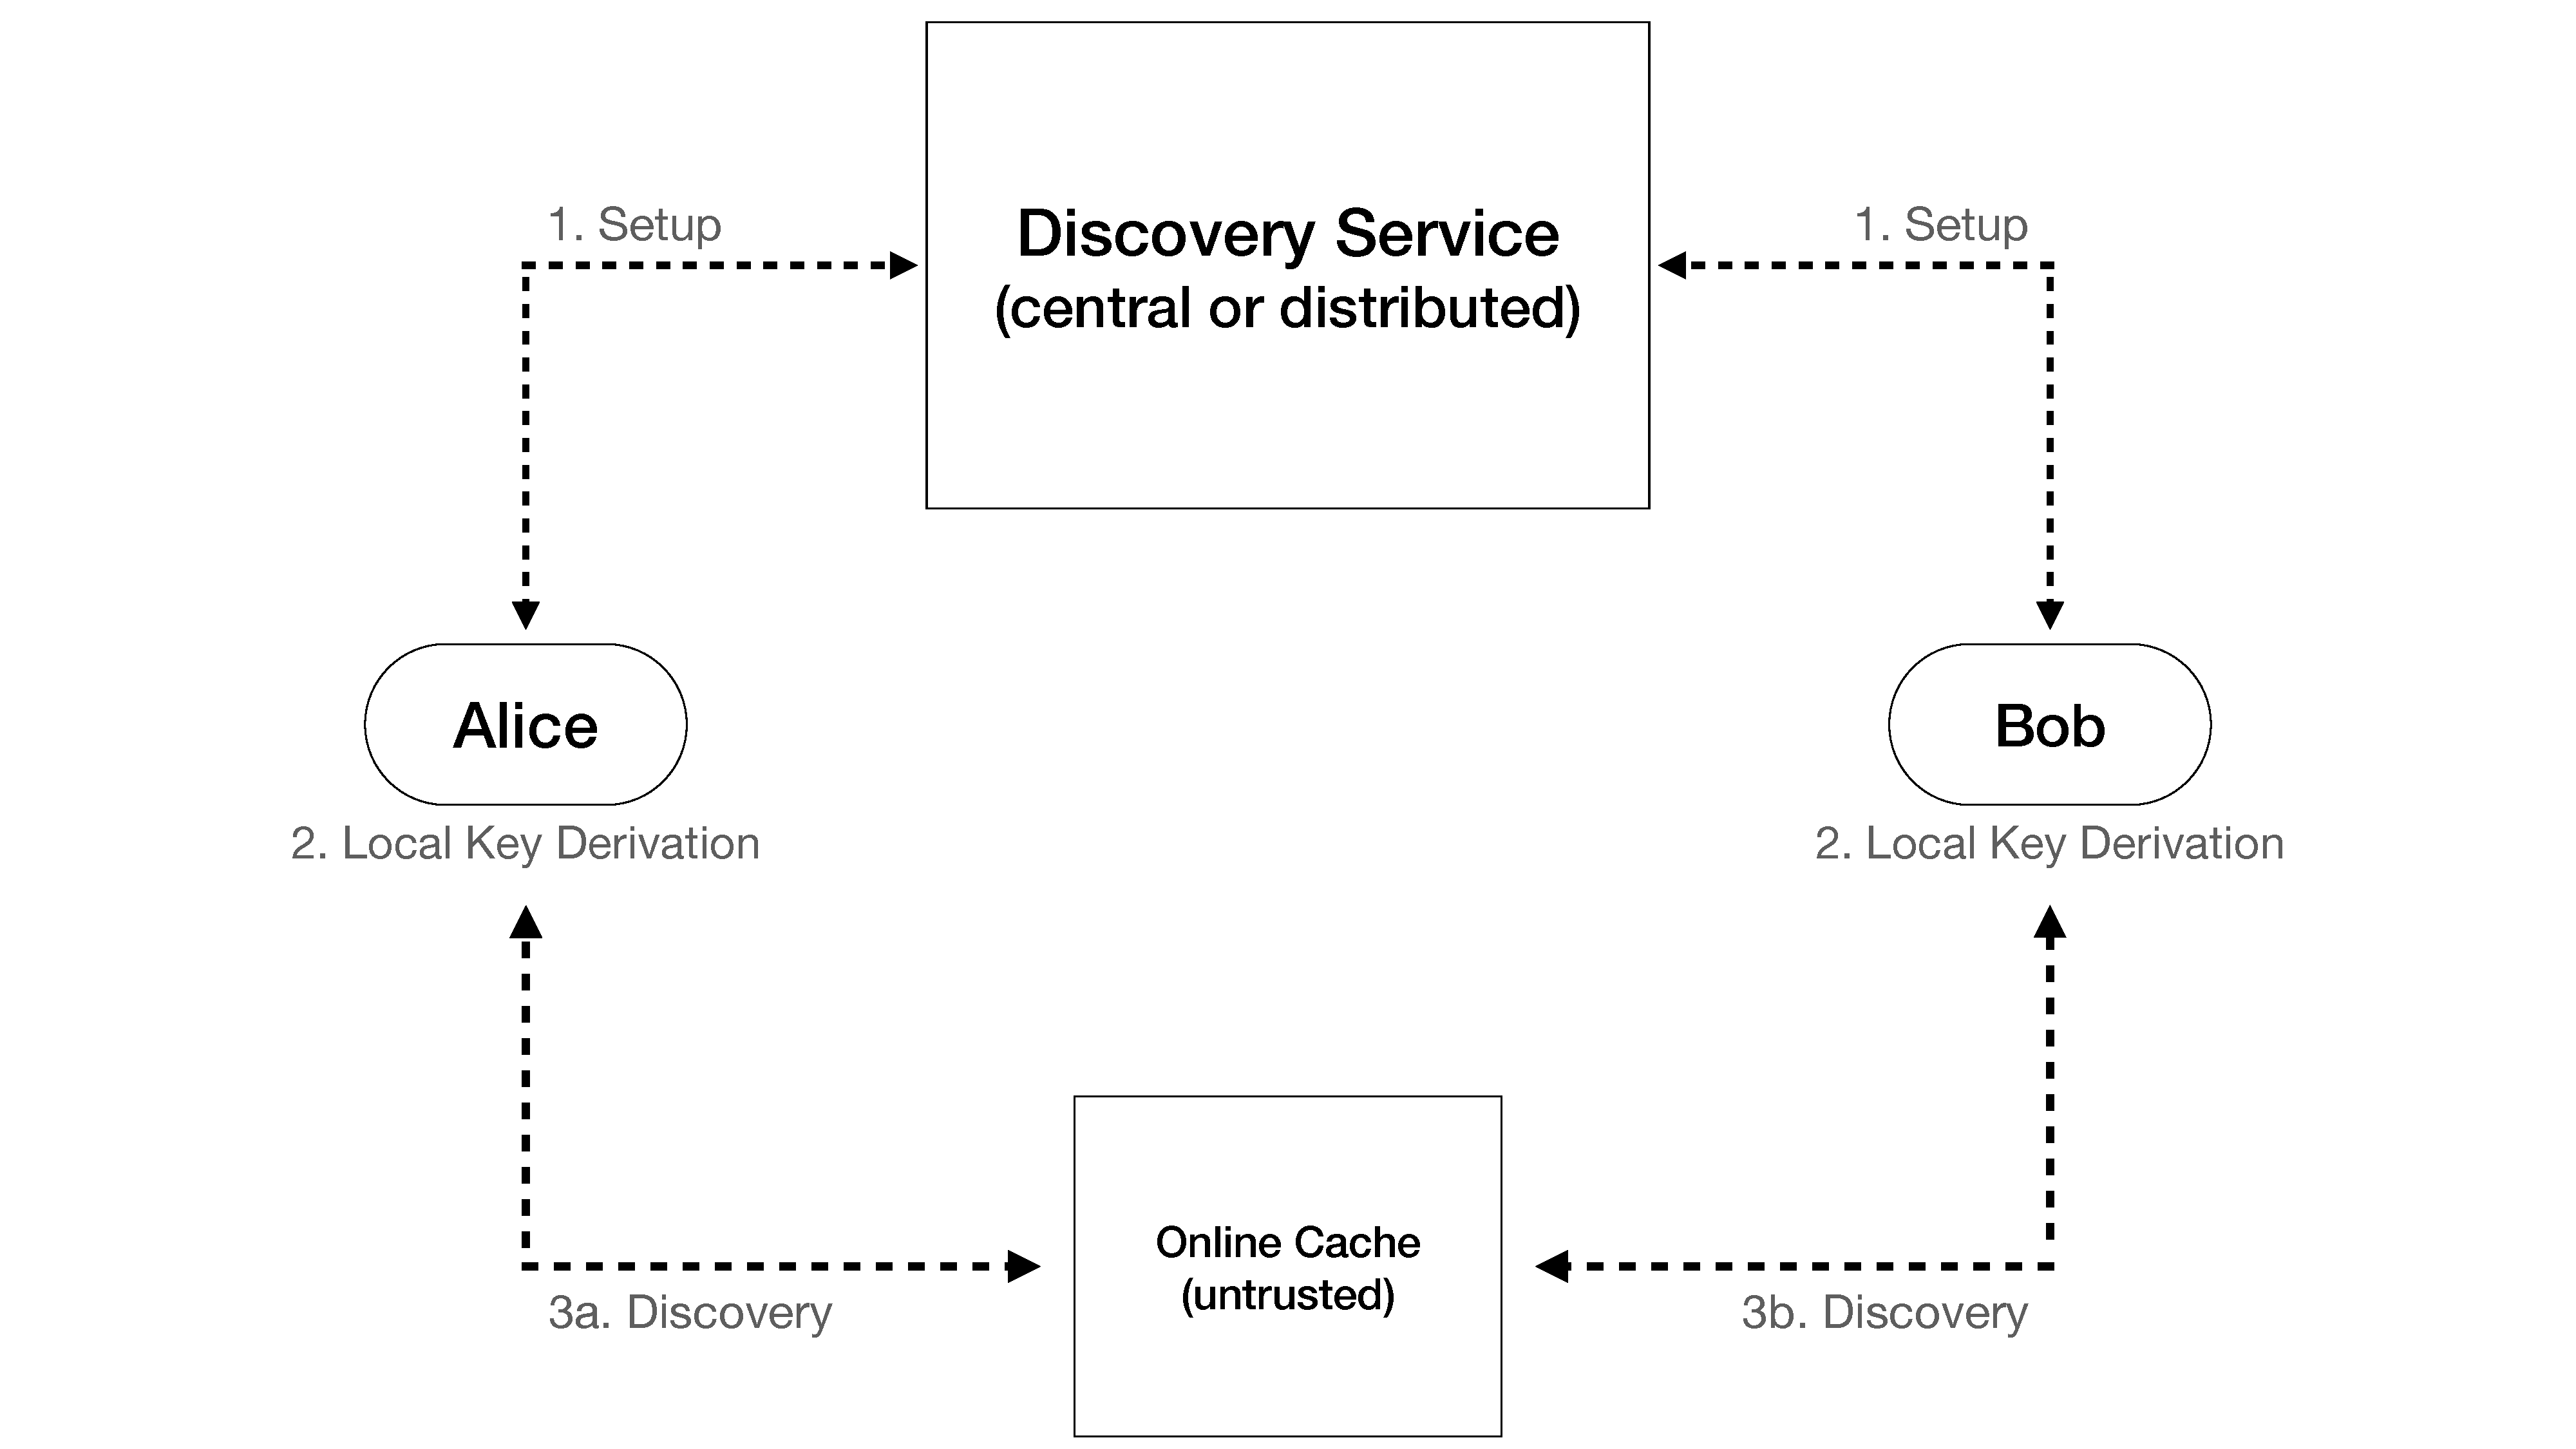
\includegraphics[width=\textwidth]{figures/system}
	  \caption{Contact discovery between a pair of users Alice and Bob, including setup. Numbers indicate the order of execution}
	  \label{fig:diagram}
	 \end{center}
 \end{figure}

	\subsection{Actors, assets and notation}
	
		\noindent We make a brief aside to clarify the actors and assets present in our scheme:		
		\begin{itemize}
			\item \textbf{Users:} each user $A$ hold a \textbf{key pair} $(\sk_A, \pk_A)$ provided by her mobile application. Furthermore, $A$ holds a \textbf{discovery identifier} $\id_A$ which could be a phone number, an email address or a username. We represent $A$'s \textbf{address book} as a set of discovery identifiers $\mathcal{ID}_A$, which is itself a subset of the set of all possible discovery identifiers $\mathcal{ID}$. Finally, we assume that users exchanged discovery identifiers through out-of-bound communication but are unable to exchange cryptographic material, including their public keys.
			\item \textbf{Discovery Service:} the discovery service $S$ may be a central or distributed entity (in the latter case we denote the set of all servers as $\mathcal{S}$ and the $i$-th server as $S_i$). In the centralised version, the discovery service holds a master secret key pair $\msk$. In the distributed version, each server holds a share of the master secret key $\msk_i$.
			\item \textbf{Online Cache:} the online cache may be operated by the discovery scheme or by a third party and is assumed to be untrusted. Its role is to manage key-value pairs.
			
			\end{itemize}
			
		\noindent Next we define the cryptographic setting for our scheme:
		\begin{itemize}
			\item $q$ is a prime of $\kappa$ bits
			\item $\Gzero, \Gone, \Gt$ are three cyclic groups of order $q$ such that there exists a pairing $e : \Gzero \times \Gone \rightarrow \Gt$.
			\item $H_0$ and $H_1$ are two public hash functions modelled as random oracles such that $H_0: \mathcal{ID}\rightarrow \Gzero$ and $H_1: \mathcal{ID} \rightarrow \Gone$.
			\item $F: \mathcal{ID}^2 \times \mathbb{Z}_q \rightarrow \Gt$ is a left/right constrained PRF defined as: \begin{equation}
				F(k, (\id_A, \id_B)) = \Pair{H_0(\id_A)}{H_1(\id_B)}^k
			\end{equation}
			\item $\mathbf{KDF}$ is a public, deterministic key derivation function.
			\item The master secret key $\msk$ is set to an element $s \in \mathbb{Z}_q$ chosen uniformly at random. In the distributed variant, we assume that the master secret key is shared according to a secure $t$-out-of-$n$ secret sharing scheme and that no single entity holds the master secret key.
		\end{itemize}

	\subsection{Key derivation}
	
		\paragraph{} We first introduce the core key derivation step even though it is performed after the setup step. In doing so, we provide the reader with the necessary material to understand the security constraints under which the setup phase operates.
		
		\paragraph{} For all users $B \in \mathcal{ID}_A$, user $A$ can compute shared key material with $B$ by evaluating $F(\msk, (\id_A, \id_B))$ and $F(\msk, (\id_B, \id_A))$. From the definition of left/right constrained PRFs, $A$ can do so with the constraining keys $\keyleft{\id_A}$ and $\keyright{\id_A}$:
		\begin{align}
			F(\msk, (\id_A, \id_B)) &= \Pair{\keyleft{\id_A}}{H_1(\id_B)} \\
			F(\msk, (\id_B, \id_A)) &= \Pair{H_0(\id_B)}{\keyright{\id_A}}
		\end{align} 
	
	\noindent Similarly, $B$ can evaluate $F$ at the same points using the constraining keys $\keyleft{\id_B}$ and $\keyright{\id_B}$:		
		\begin{align}
			F(\msk, (\id_A, \id_B)) &= \Pair{H_0(\id_A)}{\keyright{\id_B}} \\
			F(\msk, (\id_B, \id_A)) &= \Pair{\keyleft{\id_B}}{H_1(\id_A)} 
		\end{align}
	
\noindent Using this key material, $A$ and $B$ can establish a symmetric secret key using a standardised key derivation function:
	\begin{equation}
		k_{AB} = k_{BA} = \mathbf{KDF}\left(F(\msk, (\id_A, \id_B)), F(\msk, (\id_B, \id_A))\right)
	\end{equation}
	
	\paragraph{A note on security --} The constraining keys $\keyleft{\id_A}$ and $\keyright{\id_A}$ allow to compute every symmetric key that $A$ may establish with her contacts. As such, those \textbf{constraining keys must remain private} to $A$. The consequences of a leak range from impersonation to a total leak of $A$'s address book and are further detailed in \autoref{sec:security}.
	
	\subsection{Setup}
	\label{sec:setup}
		
		\paragraph{}  The setup stage serves to provide user $A$ with the constraining keys $k_{\id_A,\mathrm{LEFT}}$ and $k_{\id_A,\mathrm{RIGHT}}$. Consequently, the setup is a security-critical task. As we have shown in \autoref{eq:constrkeys}, under our construction of $F$ the constraining keys can be expressed as:
		\begin{equation}
			k_{\id_A,\mathrm{LEFT}} = H_0(\id_A)^\msk \quad \mathrm{and} \quad k_{\id_A,\mathrm{RIGHT}} = H_1(\id_A)^\msk
		\end{equation}
		
		\noindent These constraining keys can be seen as BLS signatures by the discovery service on $A$'s discovery identifier. Notice that the service needs to produce signatures under both variants of the BLS scheme: one with signatures in $\Gzero$ and one with signatures in $\Gone$.
	
	
	\subsection{Discovery}


\section{Security}
\label{sec:security}

	\subsection{Outlines of security proofs}

	\subsection{Consequences of a breach}
	
	\subsection{Authentication: an open problem}


\section{Theoretical performance evaluation}
\label{sec:performance}


\section{Applications}
\label{sec:applications}

	\subsection{End-to-end encrypted messaging}
	
	\subsection{Mobile-first cryptocurrencies}
